% Copyright(C) 2011-2015 Pedro H. Penna <pedrohenriquepenna@gmail.com>
%
% This file is part of Nanvix.
%
% Nanvix is free software; you can redistribute it and/or modify
% it under the terms of the GNU General Public License as published by
% the Free Software Foundation; either version 3 of the License, or
% (at your option) any later version.
%
% Nanvix is distributed in the hope that it will be useful,
% but WITHOUT ANY WARRANTY; without even the implied warranty of
% MERCHANTABILITY or FITNESS FOR A PARTICULAR PURPOSE. See the
% GNU General Public License for more details.
%
% You should have received a copy of the GNU General Public License
% along with Nanvix. If not, see <http://www.gnu.org/licenses/>.

\documentclass[10pt,a4paper]{article}

% Input.
\usepackage[utf8]{inputenc}
\usepackage[english]{babel}

% Figures.
\usepackage{graphicx}
\usepackage{subcaption}

% References.
\usepackage[backend=biber]{biblatex}
\bibliography{references}

% Booksmarks.
\usepackage[bookmarks=true,hidelinks]{hyperref}

% Tables.
\usepackage{booktabs}
\usepackage{multirow}
\newcommand{\specialcell}[2][c]%
{\begin{tabular}[#1]{@{}c@{}}#2\end{tabular}}

% Abbreviations.
\newcommand{\ie}{\textit{ie.\ }}

% Dummy text.
\usepackage{lipsum}

\author{Pedro H. Penna}
\title{The Nanvix Operating System}

\begin{document}

\maketitle

\section{Introduction}
\label{section: introduction}

% About Nanvix.
Nanvix is an operating system created by Pedro H. Penna for educational purposes. It was designed from scratch to be small and simple, and yet modern and fully featured, so that it could help enthusiasts in operating systems, to learn about kernel hacking. The first release of Nanvix came out in early 2011, and since then the system has undergone through several changes. This paper details the internals of Nanvix 1.2. All previous and future releases are available at \url{github.com/ppenna/nanvix}, under the GPLv3 license.

% Paper organization.
In this section, we present an overview of Nanvix, starting with the system architecture, then presenting the system services, and finally discussing the required hardware to run the system. In later sections, we present a more detailed description of Nanvix.

\subsection{System Architecture}
\label{section: system architecture}

% Nanvix and System V.
The architecture of Nanvix is outlined in Figure \ref{figure: nanvix architecture}. It presents a similar structure to Unix System V, and it has been intentionally designed to be so due to two main reasons. First, some successful operating systems, such as Aix, Linux and Solaris, are based on this architecture. Second, System V has earned Dennis Ritchie and Kenneth Thompson the 1983 Turing Award. These points indicate that System V is a well-structured system, thus serving as a good baseline design for a new educational operating system, such as Nanvix.

% Architecture overview.
Nanvix is structured in two layers. The kernel, the bottom layer, seats on top of the hardware and runs in privileged mode, with full access to all resources. Its job is to extended the underlying hardware so that: (i) a more pleasant interface, which is easier to program, is exported to the higher layer; and (ii) resources can be shared among users, fairly and concurrently. The userland, the top layer, is where user software run in unprivileged mode, with limited access to the hardware, and the place where the user itself interacts with the system.

% Kernel architecture.
The kernel presents a monolithic architecture, and it is structured in four subsystems: the hardware abstraction layer; the memory management system; the process management system; and the file system. The hardware abstraction layer interacts directly with the hardware and exports to the other subsystems a set of well defined low-level routines, such as those for dealing with IO devices, context switching and interrupt handling. Its job is to isolate, as much as possible, all the hardware intricacies, so that the kernel can be easily ported to other compatible platforms, by simply replacing the hardware abstraction layer.

\begin{figure}[t]
	\centering
	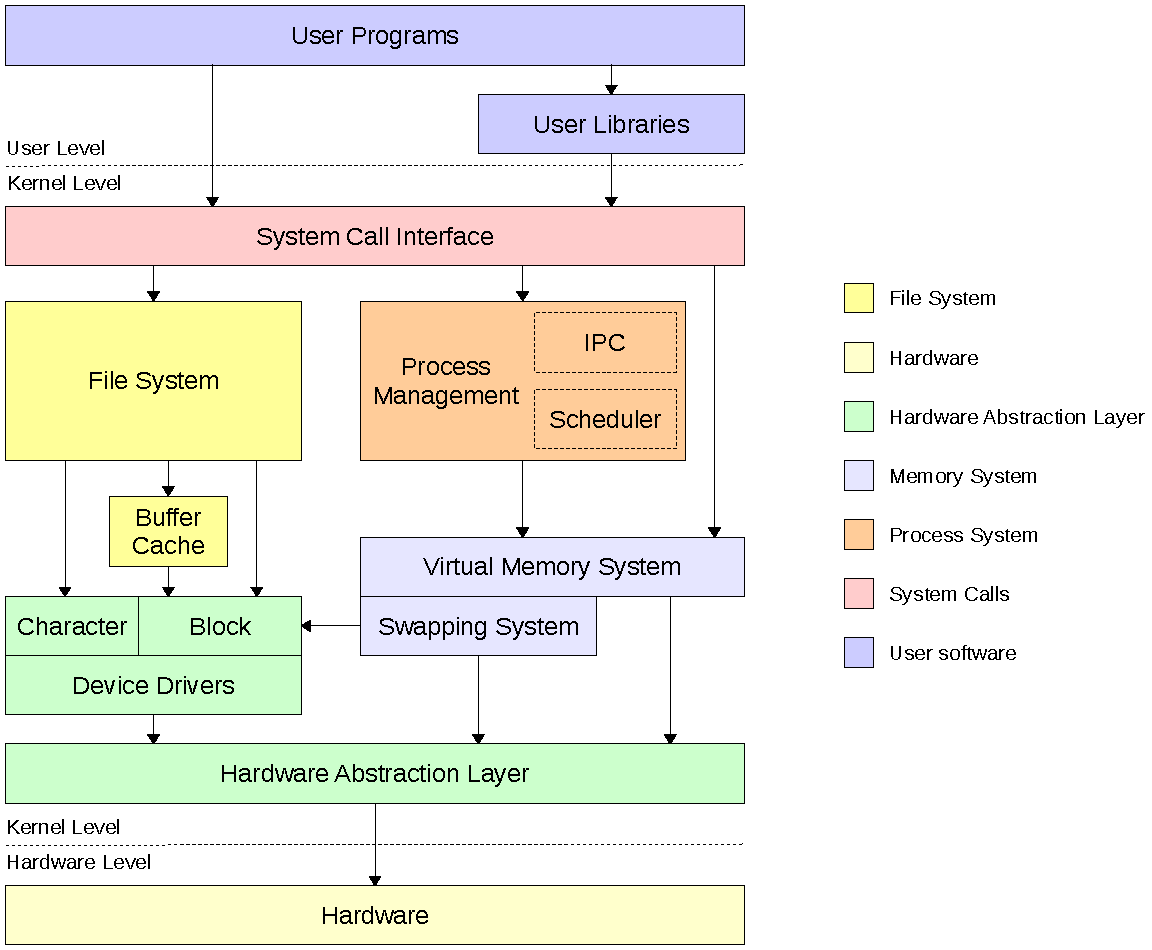
\includegraphics[scale=0.61]{img/nanvix-architecture}
	\caption{Nanvix architecture.}
	\label{figure: nanvix architecture}
\end{figure}

% Memory management system.
The memory management subsystem provides a flat virtual memory abstraction to the system. It does so by having two modules working together: the swapping and virtual memory modules. The swapping module deals with paging, keeping in memory those pages that are more frequently used and swapping out to disk those that are not. The virtual memory system, on the other hand, relies on the paging module to manage higher-level abstractions called memory regions, and thus enable advanced features such as shared memory regions, on-demand loading, lazy coping and memory pinning.

% Process management system.
The process management system handles creation, termination, scheduling, synchronization and communication of processes. Processes are single thread entities and are created on demand, either by the system itself or the user. Scheduling is based on preemption and happens in userland whenever a process runs out of quantum or blocks awaiting for a resource. In kernel land, on the other hand, processes run in nonpreemptive mode and scheduling occurs only when a processes voluntarily relinquishes the processor. Finally, processes synchronize their activities using \texttt{sleep()} and \texttt{wakeup()} primitives, and communicate with one another through pipes and signals.

% File system.
The file system provides a uniform interface for dealing with resources. It extends the device driver interface and creates on top of it the file abstraction. Files can be accessed through a unique pathname, and may be shared among several processes transparently.   The file system is compatible with the one present in the Minix 1 operating system, it adopts an hierarchical inode structure, and supports mounting points and disk block caching.

% Userland.
The userland relies on the system calls exported by the kernel. User libraries wrap around some of these calls to provide interfaces that are even more pleasant to programmers. Nanvix offers great support to the Standard C Library and much of the current development effort is focused on enhancing it. User programs are, ultimately, the way in which the user itself interacts with the system. Nanvix is shipped out with the Tiny Shell (\texttt{tsh}) and the Nanvix Utilities (\texttt{nanvix-util}), which heavily resemble traditional Unix utilities. 

\subsection{System Services}
\label{section: system services}

% System calls overview.
The main job of the kernel is to extend the underlying hardware and offer the userland a set of services that are easier to deal with, than those provided by the bare machine. These services are indeed exported as system calls, which user applications invoke just as normal functions and procedures. Nanvix implements 45 system calls, being the majority of them derived from the Posix 1 specification \cite{IEEE:08}. The most relevant system calls that are present in Nanvix are listed in Table \ref{table: most relevant system calls in nanvix}. In the paragraphs that follow, we briefly discussed each of them. For further information about system calls in Nanvix, refer to the system man pages.

% File system system calls: manipulating files.
Files are high-level abstractions created for modeling resources, being primarily designed and used to provide a natural way to manipulate disks. One program that wants to manipulate a file, shall first open it by calling \texttt{open()}. Then, it may call \texttt{read()} and/or \texttt{write()} to read and/or write data to the file. If the file supports random access, the read/write file offset may be moved through the \texttt{lseek()} system call. Finally, when the program is done with that file, it may explicitly close it by calling \texttt{close()}, and have its contents flushed to the underlying device.

% File system system calls: manipulating the file system.
Files are organized hierarchically, in a tree-like structure, and are uniquely identified by their pathnames. Programs may refer to them either by using an absolute pathname, which starts in the root directory; or by using an relative pathname to the current working directory of the program. Programs may change their current working directory by invoking \texttt{chdir()}. Alternatively, users can create links to files by calling \texttt{link()}, and then refer to the linked file by referring to the link (Figure \ref{figure: link system call}). Links and files may be destroyed through the \texttt{unlink()} system call.

% File system system calls: file permissions.
Every file has a owner user and a 9-bit flag assigned to it. These flags state what are the read, write and execution permissions for the file, for the owner user, the owner's group users and all others. If a program wants to perform any of these operations it must have enough permissions to do so. The file ownership and permissions may be changed through the \texttt{chown()} and \texttt{chmod()} system calls, respectively, and users can query these information by calling \texttt{stat()}.

\begin{figure}[b]
	\centering
	\begin{subfigure}[b]{0.35\linewidth}
		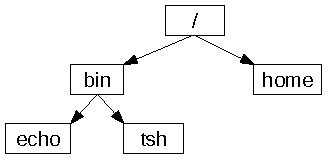
\includegraphics[width=\textwidth]{img/link-1}
		\caption{Before.}
	\end{subfigure} ~ 
	\begin{subfigure}[b]{0.35\linewidth}
		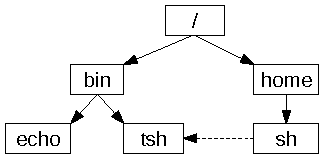
\includegraphics[width=\textwidth]{img/link-2}
		\caption{After.}
	\end{subfigure}
	\caption{\texttt{link()} system call.}
	\label{figure: link system call}
\end{figure}

% Process management system calls: dealing with processes.
Processes are abstraction of running programs and play a central role in Nanvix. Programs may create new processes by calling \texttt{fork()}, which creates an exact copy of the current running process. The primal process is called the parent and the new process is called child, and they have the same code, stack and data segments, opened files and execution flow, differing only differ in their ID number. Processes may query about their ID by calling \texttt{getpid()} and may change their core through the \texttt{execve()} system call. When the process is done, it invokes \texttt{exit()} to relinquish all resources that it was using.

% Process management system calls: signals and synchronization.
Processes may synchronize their activities using two approaches: through signals or synchronization primitives. In the former, the intend recipient process A first registers a callback function that will handle some specific signal, by calling \texttt{signal()}. If the process has nothing more to do than waiting for a signal to arrive, it may invoke \texttt{pause()} to block until such event happens. Later, another process may send a signal to A by calling \texttt{kill()}, triggering the handler function in A. In the second approach, two processes may open a pipe, a dedicate communication channel, and effectively exchange data with one another. A process in one end of the pipe writes data to it, and in the other end a second processes reads data from the pipe, with the required producer-consumer synchronization being handled by the kernel.

\begin{table}[t]
\small
\centering
\caption{Most relevant system calls that are present in Nanvix.}
\label{table: most relevant system calls in nanvix}
\begin{tabular}{l l l}
	\toprule
	Category & System Call & Description \\
	\midrule
	\multirow{12}{*}{File System}        
	                                     & \texttt{chdir}    & Changes the current working directory           \\
	                                     & \texttt{close}    & Closes a file descriptor                        \\
	                                     & \texttt{chmod}    & Changes the file permissions                    \\
	                                     & \texttt{chown}    & Changes the file ownership                      \\
	                                     & \texttt{ioctl}    & Device control                                  \\
	                                     & \texttt{link}     & Creates a new link to a file                    \\
	                                     & \texttt{lseek}    & Moves the read/write file offset                \\
	                                     & \texttt{open}     & Opens a file descriptor                         \\
	                                     & \texttt{read}     & Reads from a file                               \\
	                                     & \texttt{stat}     & Gets the status of a file                       \\
	                                     & \texttt{unlink}   & Removes a file                                  \\
	                                     & \texttt{write}    & Writes to a file                                \\
	\midrule
	\multirow{7}{*}{\specialcell{Process\\Management}}
	                                     & \texttt{execve}   & Executes a program                              \\
	                                     & \texttt{exit}     & Terminates the current process                  \\
	                                     & \texttt{fork}     & Creates a new process                           \\
	                                     & \texttt{getpid}   & Gets the process ID                             \\
	                                     & \texttt{kill}     & Sends a signal to a process                     \\
	                                     & \texttt{pause}    & Suspends the process until a signal is received \\
	                                     & \texttt{pipe}     & Creates an interprocess communication channel   \\
	                                     & \texttt{signal}   & Signal management                               \\
	\bottomrule
\end{tabular}
\end{table}

\subsection{Hardware Requirements}
\label{section: hardware requirements}

% Target architecture.
Nanvix has been primarily designed to target the \texttt{x86} architecture. Nevertheless, thanks to the hardware abstraction layer, it may be easily ported to other platforms. Still, the new platform shall meet some requirements to enable this smooth transition.

% Paging.
First, paging shall be somehow supported, since the memory management subsystem relies on this feature to enable virtual memory. Additionally, the hardware shall provide a protection mechanism that would point out whether a page fault has been caused due to a missing page or to a permission violation. Nanvix uses this information to easy the creation of new processes through the copy-on-write technique.

% Interrupts
Second, the hardware shall support interrupts. Nanvix is a preemptive system, and the hardware shall provide some clock device that would generate interrupts at regular time intervals. The scheduler completely relies on this feature, and the system would not even boot without it. Additionally, the hardware should also offer a mechanism to enable and disable interrupts. The kernel uses this feature to achieve mutual exclusion on critical regions, and thus avoid race conditions.

\section{Process Management}

% Section overview.
In this section, we take a close look in the process management subsystem. We start by first presenting the process structure itself; then highlighting how process scheduling and switching happens; and finally discussing the most important mechanisms offered by this subsystem.

\subsection{The Process Structure}
\label{subsection: the process structure}

% Process abstraction overview.
A process is an abstraction of a running program. It depicts the memory core, opened files, execution flow, access permissions, current state and every other relevant information about a program. Table \ref{table: process structure} outlines the (simplified) structure of a process in Nanvix. The information about all processes is kept in a kernel table, named the process table, and it is globally visible to all subsystems.

\begin{table}[h]
\footnotesize
\centering
\caption{Simplified structure of a process in Nanvix.}
\label{table: process structure}
\begin{tabular}{l l l}
	\toprule
	Category & Field & Description \\
	\midrule
	\multirow{3}{*}{\specialcell{Context Switch\\Information}} & \texttt{kesp}   & Kernel Stack pointer \\
	                                                           & \texttt{kstack} & Kernel Stack         \\
	                                                           & \texttt{intlvl} & Interrupt Level      \\
	\midrule
	\multirow{3}{*}{\specialcell{File System\\Information}} & \texttt{pwd}    & Current Working Directory \\
	                                                        & \texttt{ofiles} & Opened Files              \\	
	                                                        & \texttt{tty}    & Output Terminal Device    \\
	\midrule
	\multirow{2}{*}{\specialcell{General\\Information}} & \texttt{status} & Exit status                                          \\
	                                                    & \texttt{pid}, \texttt{gid}, \texttt{uid} & Process, group and user IDs \\
	\midrule
	\multirow{2}{*}{\specialcell{Memory\\Information}} & \texttt{pregs} & Code, data, stack and heap segment regions \\
	                                                   & \texttt{pgdir} & Page directory       \\
	\midrule
	\multirow{4}{*}{\specialcell{Scheduling\\Information}} & \texttt{state}    & Current state       \\
	                                                       & \texttt{counter}  & Remaining quantum   \\
	                                                       & \texttt{nice}     & Priority adjustment \\	
	                                                       & \texttt{priority} & Priority            \\
	\midrule
	\multirow{2}{*}{\specialcell{Signal\\Information}} & \texttt{received} & Received signals \\
	                                                   & \texttt{handler}  & Signal handlers  \\
	\midrule
	\multirow{2}{*}{\specialcell{Timing\\Information}} & \texttt{utime} & User CPU Time   \\
	                                                   & \texttt{ktime} & Kernel CPU Time \\
	
	\bottomrule
\end{tabular}
\end{table}

% Process table maintenance.
The process management subsystem maintains the process table. Whenever a new process is created, a new entry is added to it; and when a process terminates, the corresponding entry is erased. Nevertheless, each subsystem is in charge of maintaining their own fields in the process structure. For instance, the memory management subsystem is the one that fills up information regarding the segment regions and page directory, whereas the file system keeps track of the current working directory and opened files fields.

% Process states.
A process is created whenever a user launches a program or the system itself spawns a new daemon. After that, the new process goes through a complex lifetime before it terminates, as it is shown in Figure \ref{figure: states of a process in nanvix}. Initially this new processes is ready to execute (state 1), and it is eventually selected to run by the scheduler. At this moment, the process resumes back its execution in kernel land (state 2) and jumps to userland (state 3). There, the process performs some computation, and it may either get preempted if it runs out of quantum time (state 4), or block waiting for a resource (state 5). Either way, the process later resumes its work, and loops back on these states. When the process finally gets his job done, or it somehow crashes, it terminates and becomes a zombie process (state 6). A zombie process awaits to gets all resources assigned to it to be taken away by the kernel, and then it is turned in a dead process (state 7).

\begin{figure}[t]
	\centering
	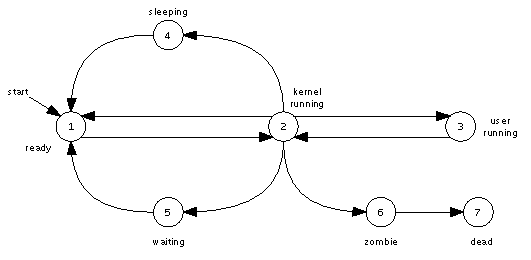
\includegraphics[scale=1.4]{img/process-states}
	\caption{States of a process in Nanvix.}
	\label{figure: states of a process in nanvix}
\end{figure}

\subsection{Process Scheduling and Switching}

% Process scheduling overview.
Several processes may be active in the system, but only one can be running at a time\footnote{Nanvix does not support multiprocessor systems, thus processes are indeed not running in parallel.}. The scheduler chooses which process to run next whenever the running process gets preempted or blocks. In user mode, that happens when the running process runs out of quantum and gets preempted by the kernel, or else when it issues a system call. In kernel mode on the other hand, scheduling occurs only when the running process voluntarily relinquishes the processor and goes wait for a resource to be released.

% Scheduling policy.
The scheduler (Figure \ref{figure: scheduler}) uses a priority based criteria to choose the next process to run, with processes with higher priorities being scheduled to run before those with lower priorities\footnote{Nanvix adopts the Unix's priority system style, in which lower values mean higher priorities.}. Processes with equal priorities are chained in a queue and are selected in a round-robin fashion.

% Priorities of a process.
The priority of a process changes over the time and it is given by the sum of tree numbers: base priority, dynamic priority and nice value. The base priority is assigned by the kernel itself and changes as the process sleeps and wakes up from resource queues, and leaves the kernel or enters it. The dynamic priority is increased by the scheduler as the process waits longer in the ready queue. Finally, the nice value is adjusted by the users, offering them a mechanism to control which processes are more priority over others.

% Process switching.
Once the scheduler choses which process to run next, the process management subsystem performs the context switching operation. It first pushes the contents of all machine registers in the kernel stack. Then, it instructs the memory management unit hardware to switch to the address space of the selected process. Finally, the state of the machine registers are restored from the kernel stack of the selected process. The context switching operation is machine dependent and it is actually carried on by the hardware abstraction layer.

\begin{figure}[t]
	\centering
	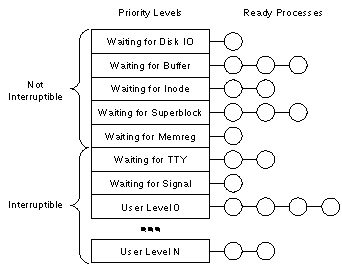
\includegraphics[scale=1.4]{img/scheduler}
	\caption{Scheduler queues.}
	\label{figure: scheduler}
\end{figure}

\subsection{Process Creation and Termination}

% Process creation.
In Nanvix, processes are created through the \texttt{fork()} system call. This call instructs the process management system to create a new process that is an exact copy of the calling process. The primal process is called the parent and the new process is called child, and they have the same code, stack and data segments, opened files and execution flow, differing only differ in their ID number. The \texttt{fork()} system call is a complex and expensive operation, and in order to get it done the process management subsystem heavily interacts with the memory management system and the file system.

% fork() in a nutshell.
First the kernel searches for an empty slot in the process table, to store there all the information about the new process. Then, a new address space for the child process is created: page tables are initialized, the kernel code and data segments are attached to the process' core, and a kernel stack for the process is created. After that, the kernel duplicates every memory region of the parent process and attaches them to the address space of the child process. In this operation, underlying pages are not actually copied, but they are rather linked and copied on demand. This technique, called copy-on-write, greatly speeds up the \texttt{fork()} system call, and it is covered in Section ??. Then, when the address space of the new process is built, file descriptors for all opened files are cloned, and every other information is handcrafted. Finally, the process management system marks the child process as new, so that the scheduler can properly handles this situation, and places it in the ready queue for later execution.

% Process termination.
The process then performs some computation and undergoes through a complex lifetime, which we depict in Section \ref{subsection: the process structure}. When the process finally finishes its job it invokes the \texttt{exit()} system call to terminate. This call orders the process management system to actually kill the process and release all resources that are assigned to it.

% exit() in a nutshell.
To do so, several steps are involved. First, the kernel masks out signals and closes all files that are still opened. After that, all child processes of the process that is about to terminate are assigned to a special process, called \texttt{init}\footnote{\texttt{init} is a daemon process whose job is to spawn the logging processes.}. This ensures that no process becomes orphan, and thus become unreachable by signals (see Section \ref{subsection: process synchronization and communication}). Then, the kernel detaches all memory regions from the dying process and marks it as a zombie. At this moment, the dying process still has an address space and a slot in the process table, and it has no way to wipe off these information. The process then hands out this task to the parent process, and sends a death of child (\texttt{SIGCHLD}) to it. This signal cannot be 
blocked or ignored, and it is eventually handled by the corresponding parent process. At this time, the parent process destroys the address space of its zombie child process, and marks the corresponding slot in the process table as not used.

\subsection{Process Synchronization and Communication}
\label{subsection: process synchronization and communication}

% Process synchronization.
In Nanvix, processes may cooperate to one another to accomplish a common goal. To enable this, the kernel provides a set of synchronization primitives, so that processes can work together without messing up each other's job. In the current version of the system, three primitives are available: \texttt{sleep()}, \texttt{wakeup()} and \texttt{wait()}.

% sleep() and wakeup() in a nutshell.
When running in kernel land, processes often need to acquire and later release resources, such as slots in the system's tables and some temporary memory. The \texttt{sleep()} and \texttt{wakeup()} routines are used under this situation to avoid race conditions in the kernel. The former puts the calling process to wait in a chain; whereas the later causes all processes that are sleeping in a process chain to be moved to the ready-to-execute scheduling queue. These routines support two different sleeping states: one that is interrupted by the receipt of signals, and another that is not. Thanks to this mechanism, users can interact with foreground processes, such as those that read/write to the terminal.

% wait() in a nutshell.
In userland, processes may coordinate their activities by through the \texttt{wait()} system call. This call causes a process to block until one of its child process terminates. When such event happens, the parent process is awaken and the exit status of the terminated child is made available to it. This information can be later parsed by the parent process, so that it can known why exactly its child process has terminated and properly handle the situation.

% Process communication.
These three mechanisms enable processes to synchronize their activities and friendly work together towards a common goal. Notwithstanding, processes also have to somehow be able to communicate with one another to exchange valuable information about their progress. Nanvix offers two main mechanisms to do that: signals and pipes.

% Signals in a nutshell.
Signals are short messages that processes can send/receive asynchronously. They are mainly used to notify about the occurrence of interesting events, such as that a process has to be killed, a remote terminal has hangup and a breakpoint has been reached. The process management subsystem exports two system calls to deal with signals: \texttt{signal()} and \texttt{kill()}. The former allows a process to actually control how signals shall be handled. A process can either choose to ignore a signal, and not be notified at all about it, or else handle a signal, by registering a callback function that will do the job. The \texttt{kill()} system call on the other hand, allows a process to raise a signal, either to another process or to itself. Additionally to these system calls, the kernel also provides a system call, named \texttt{pause()}, which allows process to wait for the receipt of a signal. Signals are implemented by having the kernel to instrument the user stack, when a signal is send. The kernel carefully inserts hooks to the registered signal handler in the stack, and when the process leaves the kernel, it transparently executes the signal handler function (Figure \ref{figure: signal stack}.

% Pipes in a nutshell.
Signals are useful for exchanging small amount of information. However, if processes want to carry on more verbose conversations, they can use pipes instead. A pipe is a virtual file that serves as a dedicated communication channel between two processes. At one end of the pipe, a writer process puts data on the pipe, and at the other end a reader processes takes data out from it. Processes can open pipes through the \texttt{pipe()} system call, and after that they can read/write data to it by using the \texttt{read()} and \texttt{write()} system calls, as they normally do. In all these operations, data transfers take place entirely in memory, with the kernel borrowing a page frame from the kernel page pool and pinning it in memory. Additionally, the kernel handles the required producer-consumer synchronization with the help of the \texttt{sleep()} and \texttt{wakeup()} routines.

\begin{figure}[b]
	\centering
	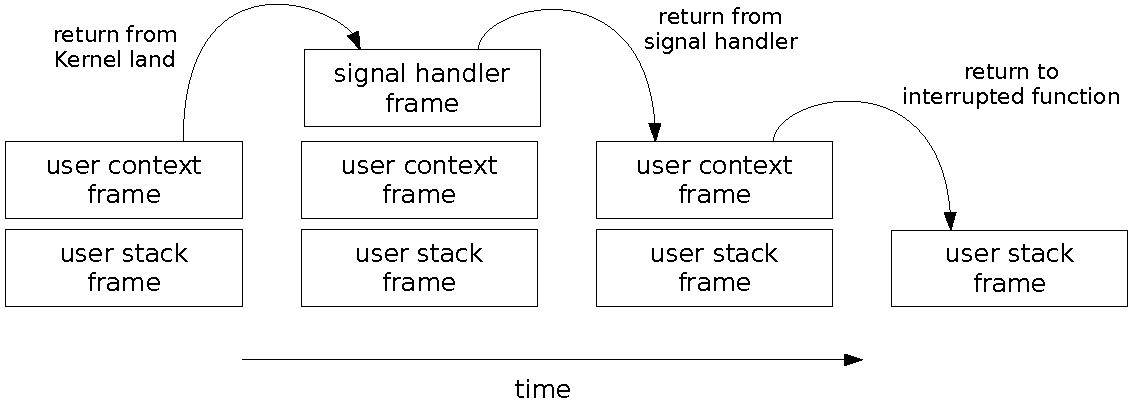
\includegraphics[scale=0.6]{img/signal-stack}
	\caption{Signal stack.}
	\label{figure: signal stack}
\end{figure}

\section{Memory Management}

% Section overview.
In this section, we detail the internals of the memory management subsystem. We first present the memory layout of a process in Nanvix, then we introduce the memory region abstraction, and finally we detail the virtual memory and paging systems.

\subsection{Memory Layout}
\label{subsection: memory layout}

% Memory layout overview.
The virtual memory layout of typical process in Nanvix is presented in Figure \ref{figure: virtual memory layout}. The overall address space is divided in two great portions: one that is owned by the kernel and is shared among all processes; and a second one that is private and belongs to the process itself. The kernel is the only one that has full access to the address space of a process. While running in user mode, if a process touches any kernel memory, a protection fault is raised. This way, the kernel can isolate and protect itself against malicious software, thus increasing the system's security and reliability.

\begin{figure}[!b]
	\centering
	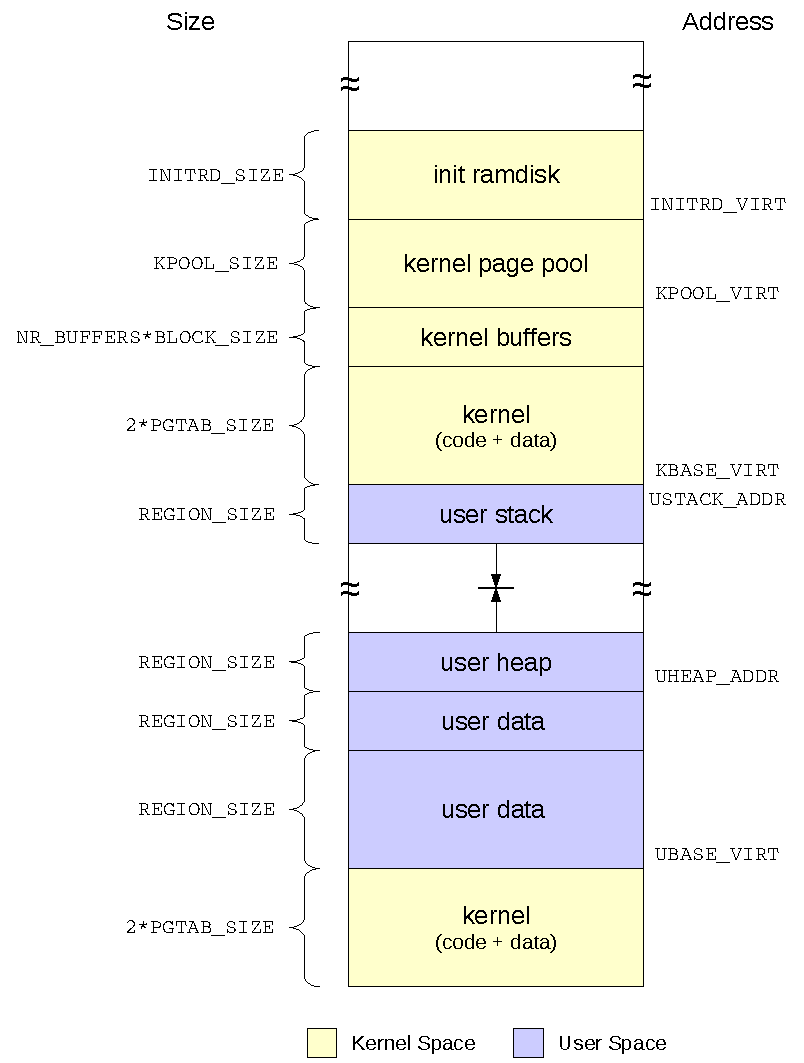
\includegraphics[scale=0.60]{img/memory-layout}
	\caption{Virtual memory layout of a process in Nanvix.}
	\label{figure: virtual memory layout}
\end{figure}

% Kernel code and data segments.
The kernel address space is carefully handcrafted so that it looks as transparent as possible to user processes. The kernel code and data segments are placed to two different locations: identity mapped at the bottom of the memory, and virtually linked just after the user memory. Some operations performed by the kernel, like physical memory copy and context switching, require the virtual memory system to be shutdown momentarily. Placing the kernel code and data segments at the bottom of the memory, enables physical address access; whereas positioning the whole kernel just after user memory ensures that future enhancements on the kernel will not affect the user memory layout.

% Kernel buffers, kernel page pool init ramdisk.
The kernel buffers, kernel page pool and init ramdisk are accessed exclusively through virtual addresses. The kernel buffer area provides the file system with some temporary memory to hold disk data. The kernel page pool feeds the kernel memory allocator with some memory that will indeed be used to build dynamic structures in the kernel, such as page tables. Finally, the init ramdisk is a static memory area that functions as a in-memory file system and stores configuration files and (eventually) dynamic loadable drivers, which are all used during system's startup.

% User memory layout.
The user memory portion occupies most of the overall virtual address space and it is divided in several regions. The user code and data regions are statically allocated and hold the text and static data segments of the binary file, respectively. The user stack and heap regions on the other hand, dynamically grow and shrink with the course of time. The former is used to store temporary variables and it is managed by the kernel's memory management subsystem. The heap region however, holds long-term variables and it is handled by the process itself. User libraries rely on the \texttt{brk()} system call to request the kernel to attach, or detach, some memory to the heap.

\subsection{Memory Regions}

\begin{figure}[!b]
	\centering
	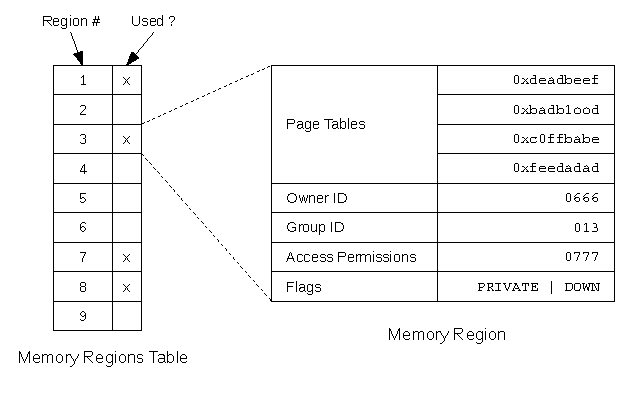
\includegraphics[scale=0.95]{img/memory-regions}
	\caption{Memory region.}
	\label{figure: memory region}
\end{figure}

% Memory regions in a nutshell.
In Section \ref{subsection: memory layout} we have seen that the user memory portion of a process is divided in four regions, namely code, data, stack and heap regions. A region is a high-level abstraction created by the memory subsystem to easy the management of user memory and abstract away the underlying technique that is used to enable virtual memory (\ie segmentation or paging). This abstraction is presented in Figure \ref{figure: memory region} and briefly discussed bellow.

% Memory regions in a paging system.
From a design perspective, a memory region is indeed a collection of page tables\footnote{The memory region abstraction equally applies to segmentation.}, with some extra metainformation about the region itself. Pointers to underlying page tables are stored in a table, so that the virtual memory and paging systems can quickly retrieve low-level information about the pages that are assigned to a region. The owner and group IDs, and access permissions fields are used together to determine what processes can read or write to the memory region. Finally, the flags field indicate the growing direction of the region, whether or not the region can be swapped out to disk, and whether or not the region is shared among several processes.

% Provided interface #1.
The memory management subsystem maintains memory regions in a global table, namely the memory regions table, and exports a well defined interface for dealing with them. The process management subsystem heavily relies on the routines provided by this interface to implement the \texttt{brk()}, \texttt{exec()}, \texttt{exit()} and \texttt{fork()} system calls, as it is outlined in Figure \ref{figure: memory regions interface}. The \texttt{allocreg()} allocates a new memory region, by searching an empty slot in the memory regions table and properly initializing its fields. It is important to point out however, that underlying pages are not actually assigned to the memory region in this routine, but they are rather allocated on-the-fly, using a technique called demand paging (see Section \ref{subsection: the virtual memory and paging systems}). Conversely, \texttt{freereg()} frees a region table by releasing underlying pages and page tables and erasing the corresponding entry from the memory regions table.

% Provided interface #2.
The \texttt{loadreg()} routine is used to load a region with some data from a binary file. This routine invokes raw I/O procedures exported by the file system to actually find the corresponding inode and perform the read operation. The \texttt{growreg()} procedure expands (or shrinks) a target region by a certain size, by allocating/freeing page tables accordingly. The \texttt{attachreg()} and \texttt{detachreg()} routines attach and detach a memory region to the address space of a process, respectively. They do so by effectively linking/unlinking underlying page tables to/from the page directory of a process. Finally, the \texttt{dupreg()} routine creates an exact copy of a target memory region. To speedup this task, the memory management subsystem uses a lazy copying technique known as copy-on-write. We further discuss this technique in Section \ref{subsection: the virtual memory and paging systems}.

\begin{figure}[!t]
	\centering
	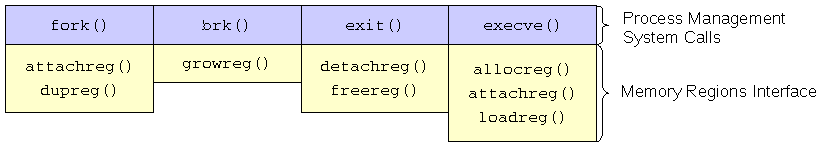
\includegraphics[scale=0.8]{img/memory-regions-interface}
	\caption{Memory regions interface.}
	\label{figure: memory regions interface}
\end{figure}

\subsection{The Virtual Memory and Paging Systems}
\label{subsection: the virtual memory and paging systems}

% Virtual memory system overview.
While the memory management system exports the memory region interface to other system modules, internally it works with paging and swapping to enable virtual memory. The former technique delivers a flat memory abstraction, whereas the latter effectively enables the physical memory to be virtually extended.

% Paging system overview.
The paging system relies on a two-level page table that is depicted in Figure \ref{figure: paging scheme} and detailed next. Each process has a single page directory, and each entry in this directory in turn points to a page table. Whenever a virtual address is generated, the memory management unit (MMU) breaks it in three portions. The upper portion is used to index the currently active page directory, and thus to find out the corresponding page table. Then, the middle portion is used to index the page table, and hence to discover the physical frame where the requested page is placed. Finally, the third portion is added to the address of the memory frame to build the ultimate target physical address.

\begin{figure}
	\centering
	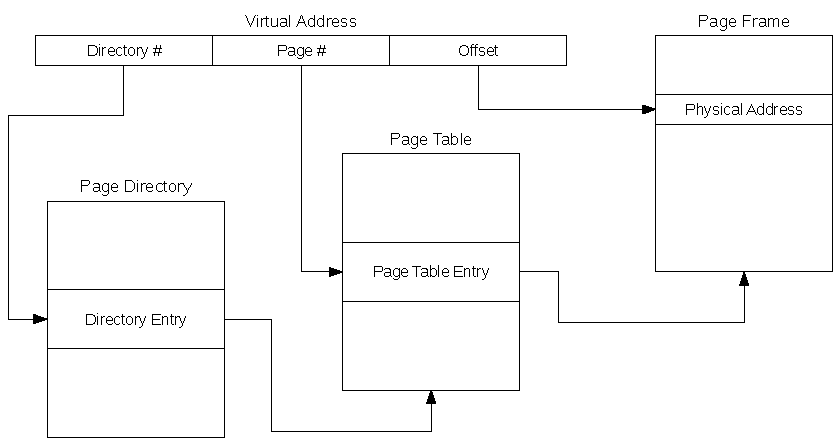
\includegraphics[scale=0.85]{img/paging-scheme}
	\caption{Two-level paging scheme used in Nanvix.}
	\label{figure: paging scheme}
\end{figure}

% Paging system internals.
Page directories and page tables of all processes are pinned down in kernel memory, and the paging system carefully bookkeeps the physical addresses of these structures. This way, the kernel can access any address space from whatever process is running, handle physical memory copying, and step away from live locks when performing swapping.

% Demand paging.
Aside from managing page directories and page tables, the paging system also implements two fundamental mechanisms: demand paging and copy-on-write. The former is extensively used in the \texttt{exec()} system call and work as follows. Whenever an executable file needs to be loaded to memory, the paging system does not copy any data from disk nor allocate any space in memory at first. Instead, it marks all corresponding entries in the page table as ``not present, demanded paging''. Later, when a attempt to access an address that falls in such kind of page is made, a page fault occurs, and then the paging system allocates a frame to that page and loads it to memory. 

% Copy-on-write.

% Page eviction.

% Swapping.

\printbibliography

\end{document}